\documentclass{article}

\usepackage{a4wide}
\usepackage[utf8]{inputenc}
\usepackage[T1]{fontenc}
\usepackage[french]{babel}
\usepackage[babel=true]{csquotes} % guillemets français
\usepackage{graphicx}
\graphicspath{{Images/}}
\usepackage{color}
\usepackage{hyperref}
\hypersetup{colorlinks,linkcolor=,urlcolor=blue}

\usepackage{amsmath}
\usepackage{amssymb}

\title{Programmation Concurrente}
\author{Jean-Emile PELLIER, L3 informatique}
\date{\today}

\begin{document}

\maketitle % pour écrire le titre

\section*{Résumé}

Il est parfois souhaitable, voire indispensable, d’effectuer certaines tâches en parallèle. Il faut alors être bien conscient que le parallélisme induit une incertitude sur l’ordre d’exécution des instructions par le processeur. Une incertitude susceptible de causer des conflits et des incohérences durant l’exécution du programme. Heureusement, il existe différents outils permettant malgré tout de s’assurer du bon fonctionnement du code ainsi exécuté.
\medbreak
Dans ce document, nous allons étudier certains de ces outils ainsi que des situations où ils sont indispensables à l’exécution cohérente d’un programme.

\section*{Introduction}

Dans un souci d’optimisation, il peut être intéressant de paralléliser certaines tâches, notamment lorsque l’on souhaite utiliser la temporisation ou lorsqu’un calcul semble trop lourd pour être effectué linéairement en temps raisonnable. Toutefois, le parallélisme n’est pas en mesure de garantir un ordre d’exécution des instructions aussi prévisible que dans le cas d’une seule tâche. Il faut alors veiller à ce que les instructions des différentes tâches agissent de manière cohérente sur les ressources qu’elles ont en commun. Afin de s’en assurer, certains procédés de \textit{synchronisation}~\cite{refSynchronisation} peuvent être plus efficaces que d’autres selon les cas.
\medbreak
Comment assurer une synchronisation optimale ?
\medbreak
Etudions deux exemples concrets, l’un en Python modélisant la gestion d’une file d’entiers, l’autre en Java modélisant des balles en mouvement.

\section*{Généralités}

Les \textit{threads}~\cite{refThread} sont un moyen d’exécuter des instructions en parallèle. On distingue deux types de threads : les threads utilisateurs et les threads daemons. Les daemons ont la particularité de s’arrêter brutalement dès lors que tous les threads utilisateurs sont terminés.
\medbreak
Afin de s’assurer que les threads s’exécutent correctement, il faut réglementer l’accès aux ressources dites critiques. L’utilisation simultanée de ces ressources par plusieurs tâches pourrait les corrompre dans la mesure où on ignore l’ordre d’exécution des instructions qui s’en servent.
\medbreak
Une idée de règlementation pertinente serait d’imposer l’ordre d’exécution en immobilisant toutes les tâches sauf une, le temps que cette unique tâche agisse sur la ressource. On peut pour cela se servir d’un verrou ou d’un sémaphore, c’est-à-dire des variables booléennes munies d’opérations \textit{atomiques}~\cite{refAtomicite} assurant aux différentes tâches un accès exclusif temporaire à la ressource critique. Cette réglementation étant bloquante, il vaut mieux éviter de monopoliser la ressource trop longtemps en s’assurant, par exemple, de minimiser la taille des blocs d’instructions atomiques.

\section{Files d'entiers}
\subsection{Interface graphique avec Tkinter}

\textit{Tkinter}~\cite{refTkinter} est une bibliothèque graphique intégrée à Python permettant la création d’interfaces graphiques portables sur les systèmes d’exploitation les plus utilisés par le grand public.
\medbreak
La création de l’interface se fait en deux temps : le paramétrage de la fenêtre et l’ajout de widgets. Tkinter dispose de la plupart des widgets usuels : les boutons, les listes, les champs de textes, etc. Une fois les widgets placés, il convient de rafraichir leur contenu périodiquement.
\medbreak
Afin d’éviter un bon nombre d’erreurs, toutes les commandes qui se rapportent à Tkinter (ou à TCL), tels que le paramétrage de la fenêtre ou des widgets, doivent être lancées dans le thread principal. La structure de Tkinter impose également d’atteindre la boucle principale (mainloop), il nous faut donc utiliser une fonction de rappel (via la méthode after) pour mettre à jour le contenu des widgets.
\medbreak
Pour créer notre application, on commence donc par créer la fenêtre principale avec la méthode Tk(), on spécifie ensuite ses dimensions. On y ajoute des widgets « Text » dont le contenu sera rafraichi au moyen de l’appel à la méthode rebuild de notre interface.
\bigbreak
\begin{center}
  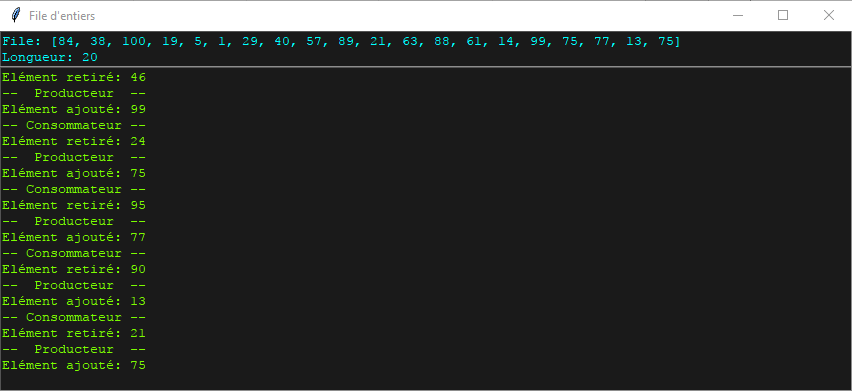
\includegraphics[scale=0.66]{File_d'entiers.png}
\end{center}
\bigbreak

\subsection{Principe}

Des threads producteurs ajoutent des nombres entiers aléatoires à une file d’entiers tandis que des threads consommateurs les retirent. L’interface affiche la file, sa longueur ainsi que les opérations effectuées sur la file. Lorsque la liste des opérations est trop longue pour être affichée sur la fenêtre, les opérations les plus anciennes sont effacées de l’écran puis envoyées vers la console qui, de fait, prolonge l’interface principale.
\medbreak
Les threads producteurs partagent un verrou avec les threads consommateurs. Ce verrou permet de s’assurer que la modification de l’interface ne peut se faire que par un thread à la fois. Ainsi, on a toujours deux lignes, la première indiquant le type du thread ayant acquis le verrou et la seconde l’opération effectuée par le thread. Remarquons que la file partagée est quant à elle protégée par Python par l’intermédiaire de l’objet \textit{Queue}~\cite{refPythonQueue} qui est « thread-safe ».

\subsection{Thread principal}

Le thread principal est rattaché à l’interface dans la mesure où Tkinter s’exécute sur ce thread. Il faut donc veiller à ne pas le bloquer afin d’éviter que l’interface ne se fige. La temporisation, les verrous ou tout autre mécanisme potentiellement bloquant sont à éviter.
\medbreak
Les \textit{fonctions de rappel}~\cite{refFonctionRappel} peuvent être utilisées pour effectuer une temporisation non bloquante.
C’est ce que permet de faire la méthode after évoquée précédemment.
\medbreak
Pour remplacer les verrous, il existe des algorithmes dits \textit{non-bloquants}~\cite{refAlgoNonBloquant} mais ils sont assez difficiles à implémenter. C’est pourquoi il est préférable d’utiliser un verrou si le nombre d’instruction dans les blocs d’instructions atomiques est faible et que le nombre de threads est peu élevé. En effet, pour un temps d’attente négligeable, le verrou n’est pas vraiment bloquant, comme dans le code suivant :
\bigbreak
Thread principal
\begin{verbatim}
   with self.verrou:
      texte = self.texte
      self.texte = ""
\end{verbatim}
\bigbreak
Threads secondaires
\begin{verbatim}
   with self.verrou:
      texte = self.texte
      self.texte = texte + txt + "\n"
\end{verbatim}

\subsection{Arrêt des threads}

Les daemons peuvent faciliter l’écriture d’un programme puisqu’ils ont un mécanisme d’arrêt automatique. Toutefois, l’arrêt s’effectuant brutalement, une mauvaise libération des ressources qu’ils utilisent est à prévoir. Il est même possible que l’interpréteur Python ignore tout simplement l’attribut daemon du thread, auquel cas le thread ne s’arrêtera pas automatiquement.
\medbreak
Une idée consiste à intercepter l’évènement de fermeture de la fenêtre pour arrêter tous les threads proprement en vérifiant au passage leurs comportements.
\medbreak
Pour cela on crée une classe qu’on appelle ThreadKiller.
\bigbreak
\begin{itemize}
\item On mémorise la liste des threads via le constructeur.
\medbreak
\begin{verbatim}
   self.th_list = th_list
\end{verbatim}
\bigbreak
\item On intercepte l’évènement de fermeture de la fenêtre avec :
\medbreak
\begin{verbatim}
   self.fenetre.protocol("WM_DELETE_WINDOW", self.terminate)
\end{verbatim}
\bigbreak
\item On crée ensuite la méthode terminate qui sera appelée à la fermeture de la fenêtre.
\bigbreak
\item On donne l’ordre d’interruption des threads répertoriés.
\medbreak
\begin{verbatim}
   for i in range(0,len(self.th_list)):
      self.th_list[i].interrupt()
\end{verbatim}
\bigbreak
\item On attend que les threads réagissent à l’ordre d’interruption, s’ils sont disposés à obéir.
\medbreak
\begin{verbatim}
   i = 0
   counter = 0
   while i<len(self.th_list):
      if not self.th_list[i].running:
         print(u"Thread %d interrompu (%d secondes)"%(i,counter))
         i = i + 1
         counter = 0
      elif self.th_list[i].waiting:
         time.sleep(1)
         counter = counter + 1
      else:
         print(u"Thread %d récalcitrant"%i)
         i = i + 1
         counter = 0
\end{verbatim}
\bigbreak
\item Et bien sûr on déclenche la fermeture de la fenêtre qu’on avait empêché.
\medbreak
\begin{verbatim}
   self.fenetre.destroy()
\end{verbatim}
\end{itemize}

\section{Balles en mouvement en Java}
\subsection{Interface graphique avec Swing}

\textit{Swing}~\cite{refSwing} offre la possibilité de créer des interfaces graphiques identiques quel que soit le système d’exploitation sur lequel on lance l’application.
\medbreak
Swing fonctionne sur un système d’assemblage de composants. Tout ce qui constitue la fenêtre est un composant, que ce soit la fenêtre elle-même ou encore les conteneurs, les boutons, les listes, les champs de textes, etc. Le thread de l’interface se charge de mettre à jour les composants automatiquement par l’appel au paintComponent du panneau.
\medbreak
On commence par créer une fenêtre par héritage sur JFrame. On paramètre la fenêtre, on y ajoute un panneau hérité de JPanel. On ajoute un autre panneau à celui-ci que l’on dispose au moyen d’un Layout afin d’y ajouter les boutons hérités de JButton au bas de la fenêtre.

\bigbreak
\begin{center}
  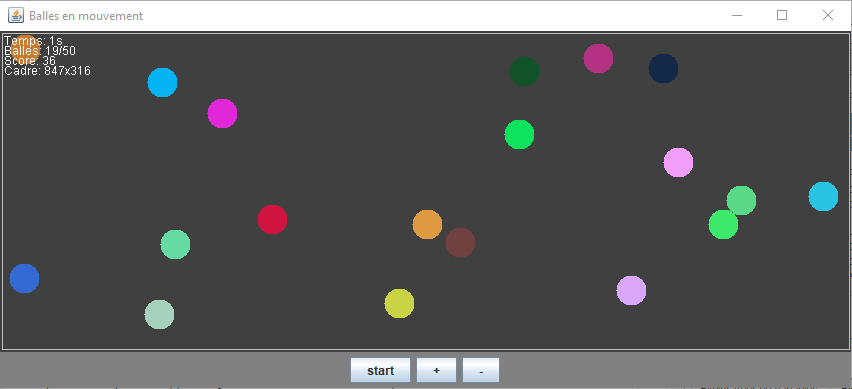
\includegraphics[scale=0.66]{Balles_en_mouvement.png}
\end{center}
\bigbreak

\subsection{Principe}

Des balles se déplacent dans une fenêtre en ricochant contre les bords. Un bouton permet de démarrer/arrêter le mouvement de toutes les balles. Les boutons + et – permettent respectivement d’ajouter ou supprimer une balle. En cas de collision, les balles impliquées sont supprimées et le score est incrémenté. Une horloge indique la durée durant laquelle les balles sont en mouvement. Les bords du cadre sont réajustés automatiquement en cas de redimensionnement de la fenêtre.

\subsection{Moteur physique}

Le moteur physique fonctionne sur un thread dédié tout comme l’horloge. D’ailleurs, c’est le moteur qui déclenche et interrompt l’horloge dans la mesure où celle-ci décrit le temps d’activité du moteur. Cette durée étant calculée en secondes, le thread de l’horloge est soumis à une temporisation fixe, d’où l’intérêt de dissocier les deux threads si on veut ajuster la vitesse de déplacement des balles.
\medbreak
Le moteur gère toutes les actions liées aux différents boutons, les mouvements ainsi que les collisions mais il sert avant tout à demander le rafraichissement de l’interface. Le rafraichissement et le dessin des balles est effectué par le thread d’affichage à travers le paintComponent du panneau.
\medbreak
Le déclenchement des actions se fait sur un autre thread via un écouteur d’évènement. Il faut donc veiller à ce que la liste des balles soit « thread-safe » d’où l’utilisation de \textit{ConcurrentLinkedQueue}~\cite{refJavaQueue}.

\section*{Conclusion}

En présence de plusieurs threads, il faut utiliser des mécanismes de synchronisation afin d’éviter que les ressources partagées ne soient altérées. Les mécanismes dits bloquants sont plus faciles à implémenter mais ils imposent d’attendre, plus ou moins longtemps, la disponibilité d’une ressource.
\medbreak
Il est important de s’assurer d’arrêter tous les threads créés puisque des tâches inutiles qui saturent le système peuvent causer des erreurs de toutes sortes ainsi que des plantages systèmes inopinés.

%%% La bibliographie:
\bibliographystyle{plain}
\bibliography{biblio}

\end{document}
